\chapter{Testy}
\label{ch:testy}

Ostatnim etapem projektu było przeprowadzenie testów, pozwalających na sprawdzenie działania wszystkich elementów systemu akwizycji danych. Przeprowadzono testy sprzętu i oprogramowania, sprawdzana była poprawność i niezawodność działania całego systemu z dołączanymi zewnętrznymi czujnikami.

 
\section{Przebieg testów}
Przeprowadzono szereg testów funkcjonalnych w celu sprawdzenia czy system spełnia założenia projektowe zawarte we wstępie pracy. 


\begin{itemize}
\item analiza częstotliwościowa z wykorzystaniem algorytmu FFT (z ang. Fast Fourier Transform - szybkiej transformaty Fouriera) sygnału sinusoidalnego z zastosowaniem odpowiedniego okna czasowego
\item sprawdzenie dokładności pomiarów przy użyciu laboratoryjnych przyrządów pomiarowych 
\item test niezawodności działania przy dużym obciążeniu aplikacji
\item sprawdzenie poprawności danych z uwzględnieniem korelacji czasowej
\item test funkcjonalny komunikacji sieciowej
\end{itemize}

\section{Użyte narzędzia}
Sprawdzenie parametrów pomiaru napięcia przetwornika analogowo-cyfrowego przeprowadzono z użyciem oscyloskopu cyfrowego z funkcją generowania przebiegów sygnałów. Fakt, iż oscyloskop był cyfrowy ułatwił analizę różnic w sygnale wyjściowym z generatora i sygnałem spróbkowanym. Pomiary na oscyloskopie przeprowadzane były z użyciem sondy oscyloskopowej. Na Rys. \ref{pic:stanowisko} przedstawiono stanowisko pomiarowe systemu akwizycji danych.

\begin{figure}[h]
	\centering
		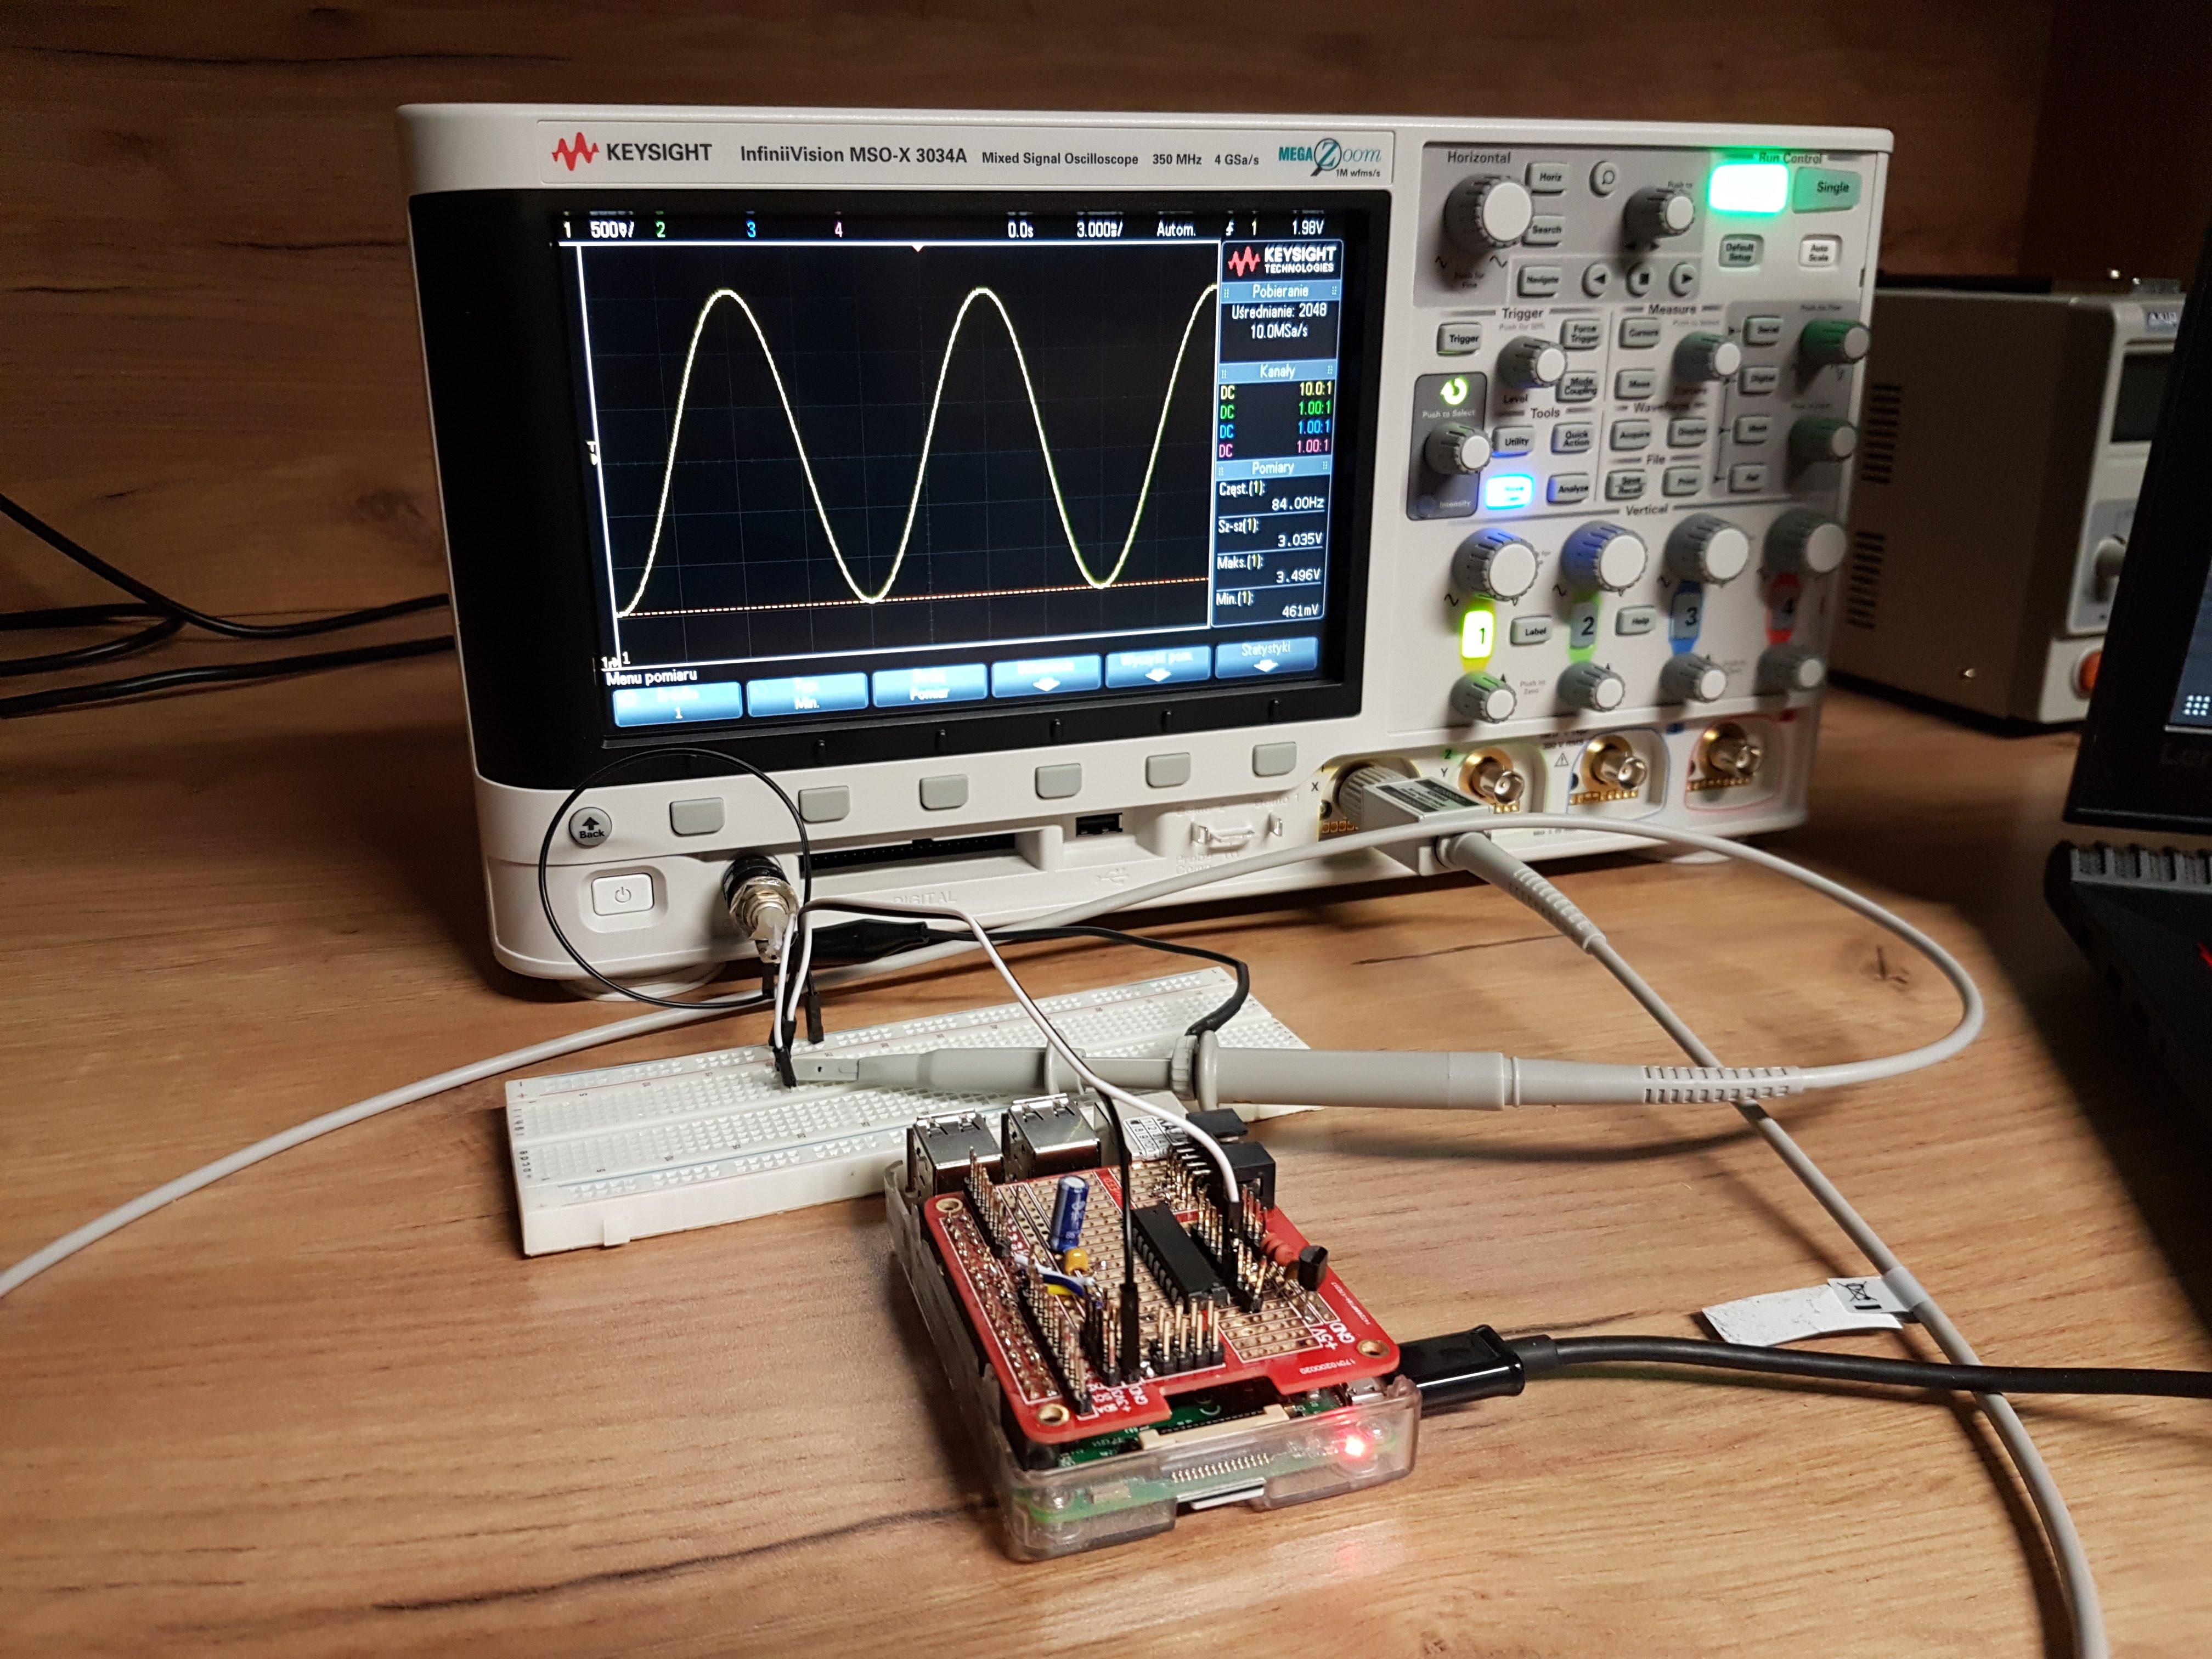
\includegraphics[width=13cm]{stanowisko}
	\caption{Stanowisko pomiarowe do pomiaru napięcia sinusoidalnego przetwornikiem analogowo-cyfrowym} 
	\label{pic:stanowisko}
\end{figure}


\section{Testy funkcjonalne}


\subsection{Test interfejsu sieciowego}

Wykonano test działania interfejsów sieciowych systemu użytkownika pod kątem spójności danych wysyłanych z systemu do użytkownika podłączonego przez sieć TCP/IP. Połączenie użytkownika korzystającego z przeglądarki w komputerze osobistym z systemem akwizycji danych było zestawione przy wykorzystaniu routera Wi-Fi.
 


\subsection{Testy niezawodności systemu}

Niezawodność działania systemu jest bardzo istotna w przypadku sieciowego systemu akwizycji danych. Urządzenie jest przystosowane do pracy autonomicznej, więc aby zdalny dostęp mógł być zapewniony, Raspberry Pi musi być w stanie wykrywać stan zawieszenia systemu, gdyż wpływa to bezpośrednio na niezawodność i ciągłość działania. 

W komputerze Raspberry Pi istnieje możliwość uaktywnienia układu \ang{watchdog}, zapewniającego automatyczny restart systemu w przypadku jego zawieszenia. 
Raspbian zawiera moduł do jądra obsługujący licznik układu \ang{watchdog}. 
Aby uaktywnić układ należy dodać parametr do drzewa urządzeń za pomocą wpisania \ang{dtparam=watchdog=on} w pliku zawierającym konfigurację ładowania systemu \cite{watchdog}. Dodatkowo w pliku /etc/modprobe.d/bcm2835-wdt.conf można zdefiniować czas braku aktywności systemu po jakim układ \ang{watchdog} wywoła ponowne uruchomienie systemu, wpisując \ang{options bcm2835\_wdt heartbeat=14 nowayout=0}. Należy stworzyć jeszcze plik /etc/modprobe.d/bcm2835-wdt.conf zawierający konfigurację modułu obsługującego układ \ang{watchdog}: \ang{options bcm2835\_wdt heartbeat=14 nowayout=0}.

Po ustawieniu odpowiedniej konfiguracji przeprowadzono testy niezawodności działania układu \ang{watchdog}, wywołując aplikacje powodujące zawieszenie systemu z załadowanym modułem. Oprócz konsoli \ang{ssh} podłączono komputer przez konwerter USB-UART w celu upewnienia się, że system jest uruchamiany ponownie.
Testy zakończono sukcesem, moduł sterujący układem \ang{watchdog} działał poprawnie i wywoływał ponowne uruchomienie systemu przy każdym zawieszeniu. 


\section{Wyniki pomiarów}


\subsection{Charakterystyki napięcia spróbkowanego przetwornikiem ADC MAX1202}

\subsubsection{Pomiar napięcia sinusoidalnego}

Pomiar napięcia sinusoidalnego i jego analiza częstotliwościowa, umożliwia sprawdzenie poziomu nierównomierności okresu próbkowania. 
Z oscyloskopu z funkcją generatora sygnałów wygenerowano przebieg sinusoidalny o częstotliwości 100Hz, amplitudzie 3Vp-p i składowej stałej 2V. Okres próbkowania przetwornika ustawiono w aplikacji testowej na 200us co przekłada się na częstotliwość próbkowania 5kHz. 
Spróbkowany sygnał został poddany analizie za pomocą algorytmu FFT przy użyciu skryptu pythona z pakietami \ang{numpy} i  \ang{matplotlib} .
Poniżej na Rys. \ref{fig:sin_max1202_100Hz_adc} przedstawiono fragment wykreślonego przebiegu czasowego sygnału sinusoidalnego. Linią przerywaną zaznaczono wartość średnią sygnału.

\begin{figure}[H]
	%\centering
		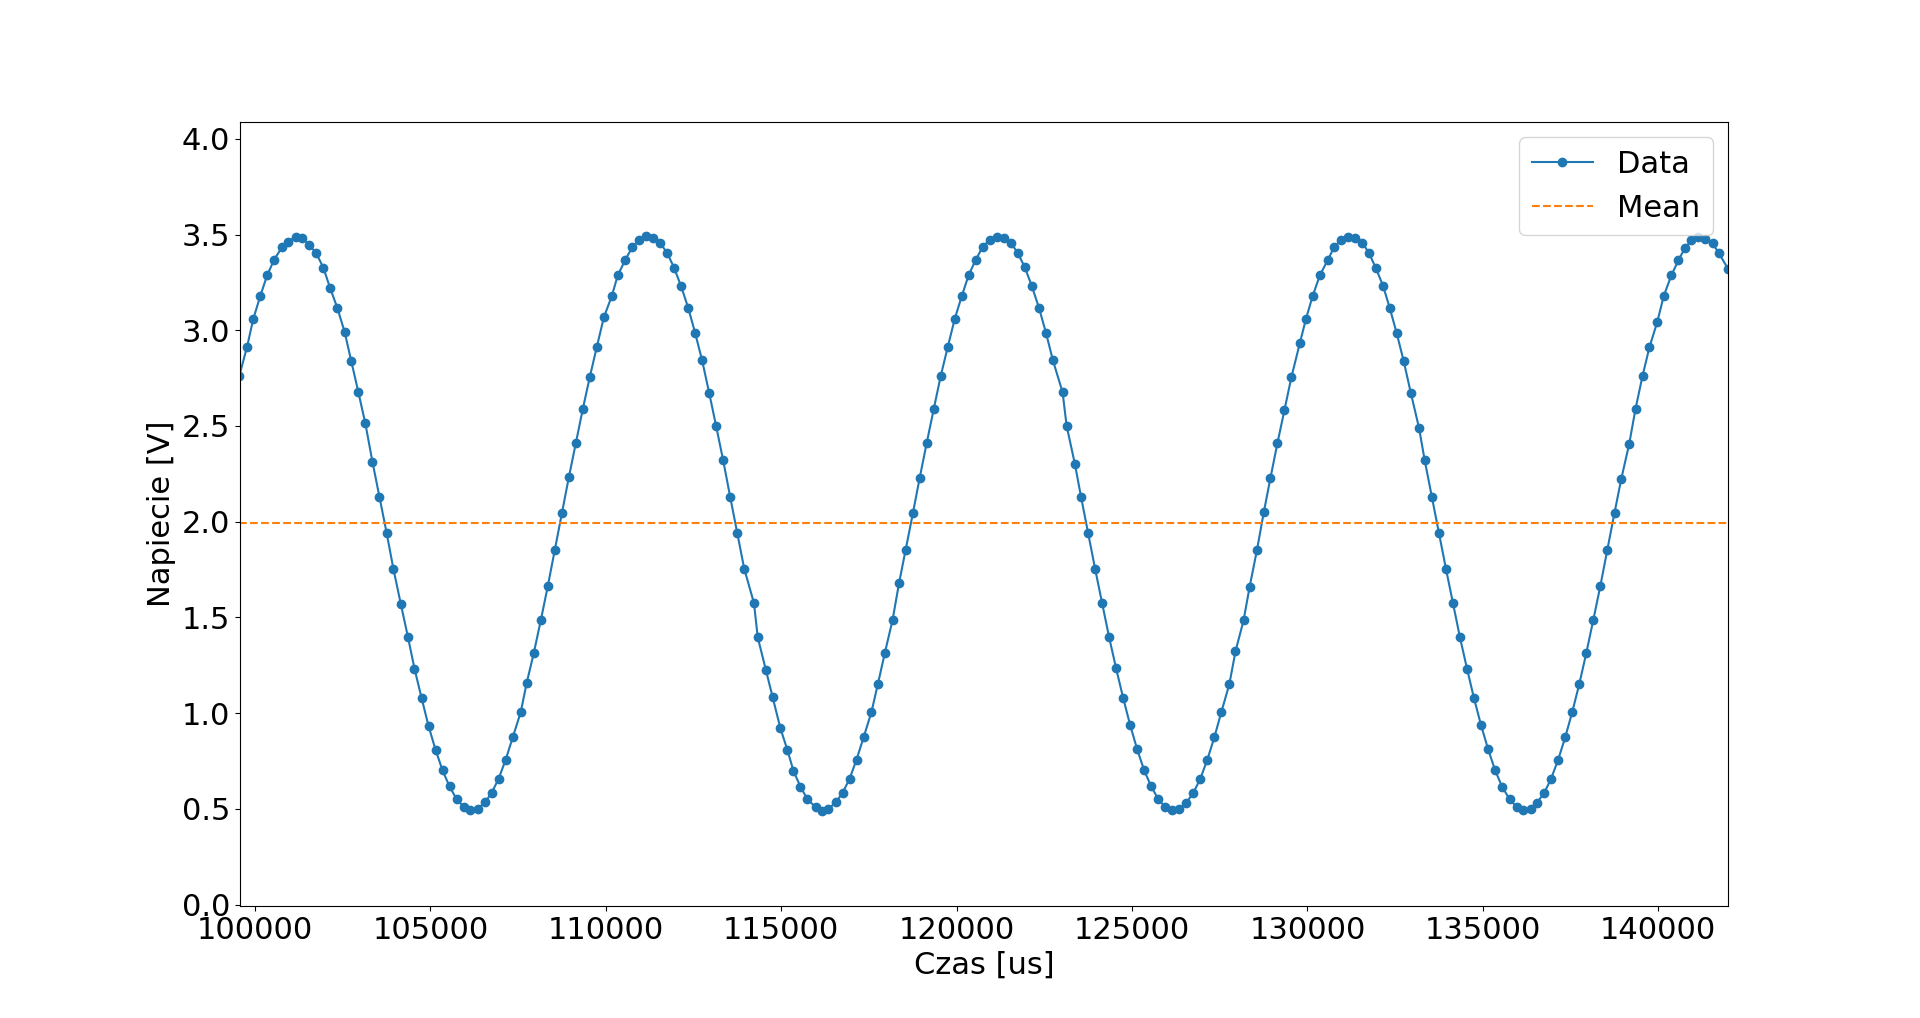
\includegraphics[width=14cm]{sin_max1202_100Hz_adc}
	\caption{Przebieg napięcia spróbkowanego przetwornika ADC MAX1202} 
	\label{fig:sin_max1202_100Hz_adc}
\end{figure}

Dla porównania sygnał z generatora zmierzono oscyloskopem przy użyciu sondy oscyloskopowej. Zrzut z ekranu oscyloskopu poniżej na Rys. \ref{fig:sin_max1202_100Hz_osc} 

\begin{figure}[H]
	\centering
		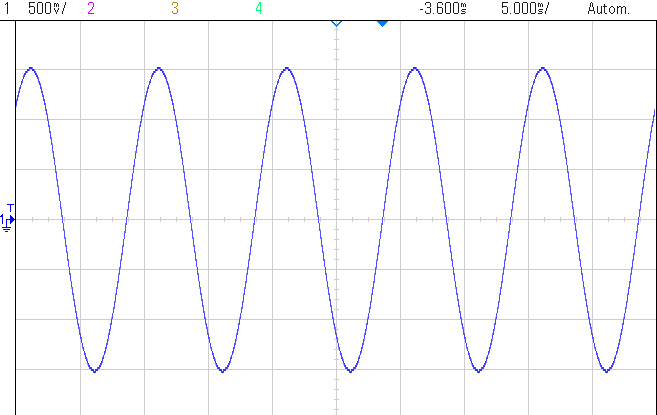
\includegraphics[width=12cm]{sin_max1202_100Hz_osc.png}
	\caption{Przebieg napięcia sinusoidalnego z oscyloskopu} 
	\label{fig:sin_max1202_100Hz_osc}
\end{figure}

Poniżej na Rys. \ref{fig:zmiennosc_probkowania_max1202} przedstawiono charakterystykę zmienności okresu próbkowania. Widać na niej jak zmienia się okres próbkowania w trakcie działania programu.

\begin{figure}[h]
	\centering
		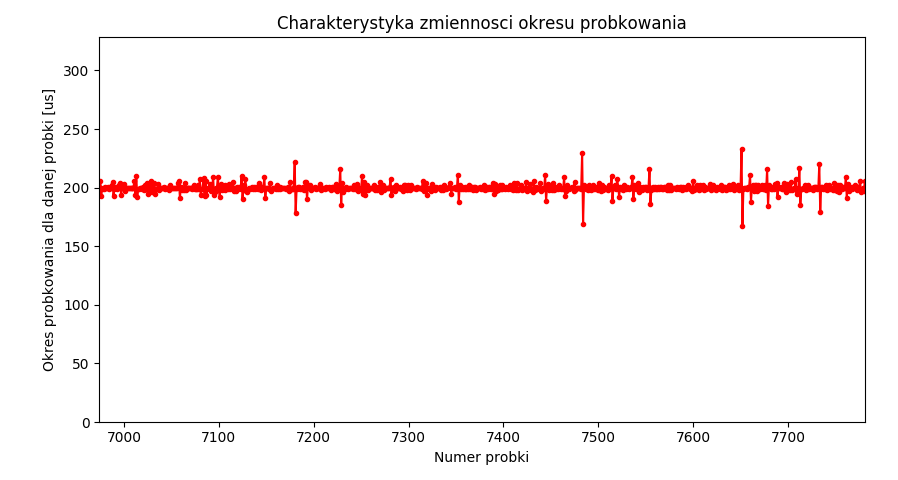
\includegraphics[width=14cm]{zmiennosc_probkowania_max1202}
	\caption{Charakterystyka zmienności okresu próbkowania przy użyciu sterownika do ADC} 
	\label{fig:zmiennosc_probkowania_max1202}
\end{figure}

Zmienność okresu próbkowania opisano przy użyciu parametru odchylenia standardowego. Wyniki z pomiaru napięcia sinusoidalnego w Tablicy 5.1.:

\begin{table}[t]
\label{tab5.1}
\centering
\begin{tabular}{|l|l|l|}
  \hline 
  Ilość zebranych próbek & 19958 \\
  \hline
  Średni okres próbkowania [$\mu$s] & 200 \\
  \hline
  Średnia częstotliwość próbkowania [Hz]& 5000 \\
  \hline 
  Wariancja okresu próbkowania [$\mu$s]  & 454 \\
  \hline
  Odchylenie standardowe okresu próbkowania [$\mu$s] & 21,3 \\
  \hline

  
\end{tabular}
\caption{Parametry opisujące zmienność okresu próbkowania} 
\end{table}


\subsubsection{Pomiar napięcia prostokątnego}

Wykonano również pomiar napięcia prostokątnego. Sygnał spróbkowano z częstotliwością 5kHz, charakterystyka jest przedstawiona na Rys. \ref{fig:rect_max1202_100Hz_adc}, a oscylogram na Rys. \ref{fig:rect_max1202_100Hz_osc} 

\begin{figure}[h]
	\centering
		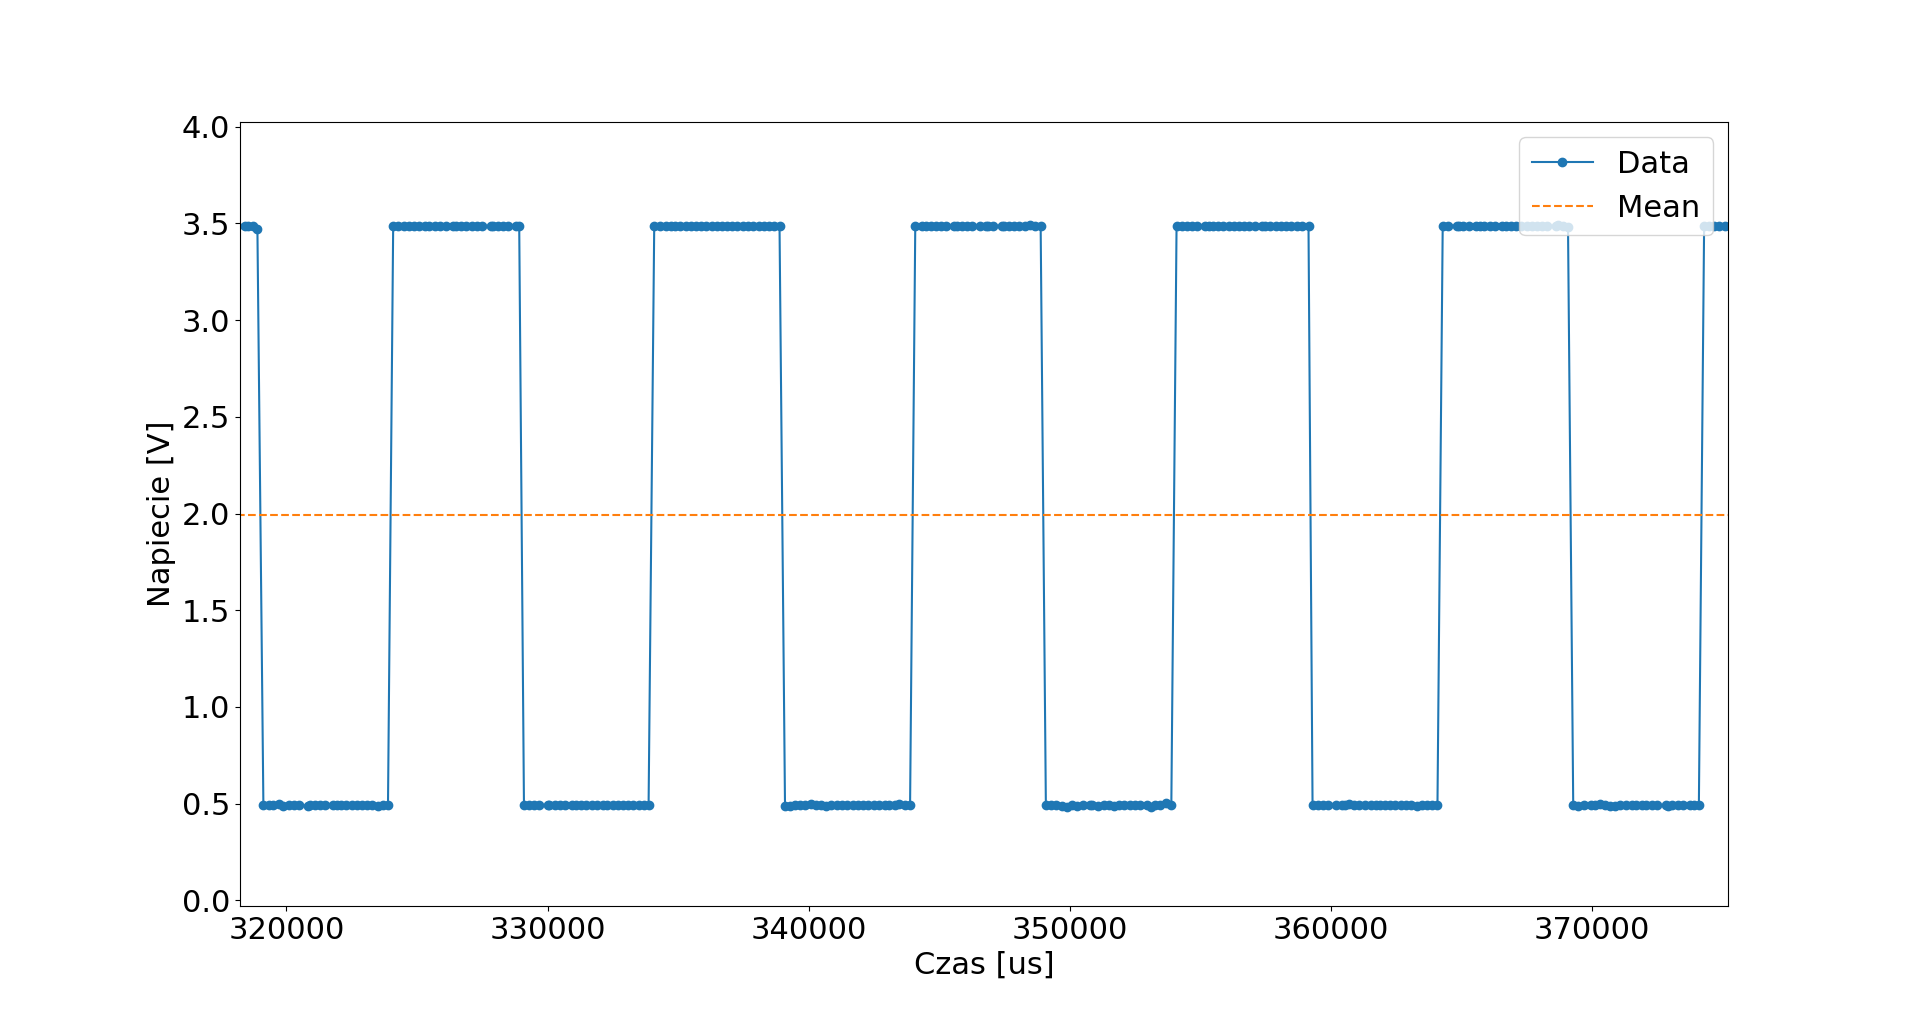
\includegraphics[width=15cm]{rect_max1202_100Hz_adc}
	\caption{Przebieg napięcia spróbkowanego przetwornika ADC MAX1202} 
	\label{fig:rect_max1202_100Hz_adc}
\end{figure}


\begin{figure}[h]
	\centering
		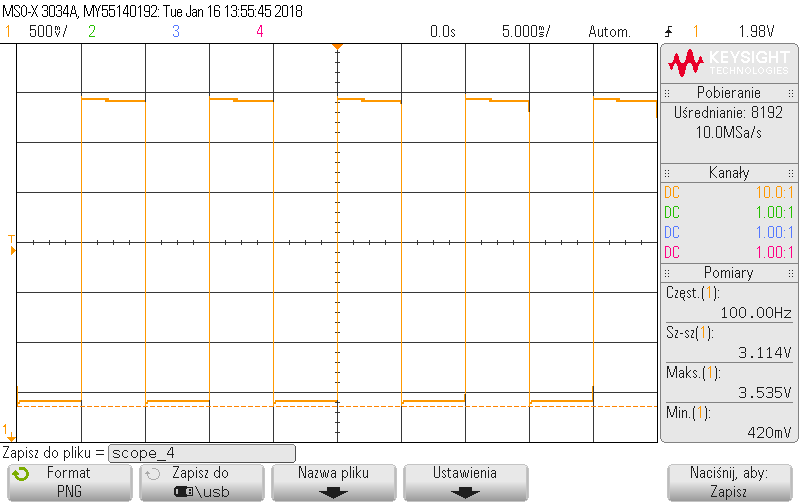
\includegraphics[width=12cm]{rect_max1202_100Hz_osc}
	\caption{Przebieg napięcia prostokątnego na oscyloskopie} 
	\label{fig:rect_max1202_100Hz_osc}
\end{figure}

\subsection{Analiza FFT sygnału sinusoidalnego}

Przed wykonaniem pomiaru dokonano symulacji komputerowej w celu dostrzeżenia różnic charakterystyk częstotliwościowych między sygnałem sinusoidalnym bez zniekształceń, a sygnałem z nierównomiernymi odstępami czasowymi pomiędzy kolejnymi próbkami. 
Sygnał został wygenerowany numerycznie, a następnie zniekształcony poprzez dodanie do wektora czasu pseudolosowych wartości z zakresu od 0 do 50us. Rysunek \ref{fig:sin_fft_ideal} przedstawia przebieg czasowy sygnału zniekształconego, jego charakterystykę częstotliwościową oraz widmo sygnału sinusoidalnego bez zniekształceń. Charakterystyki wyznaczono przy użyciu algorytmu FFT i przemnożeniu przez okno Hanninga.

\begin{figure}[H]

	\centering
		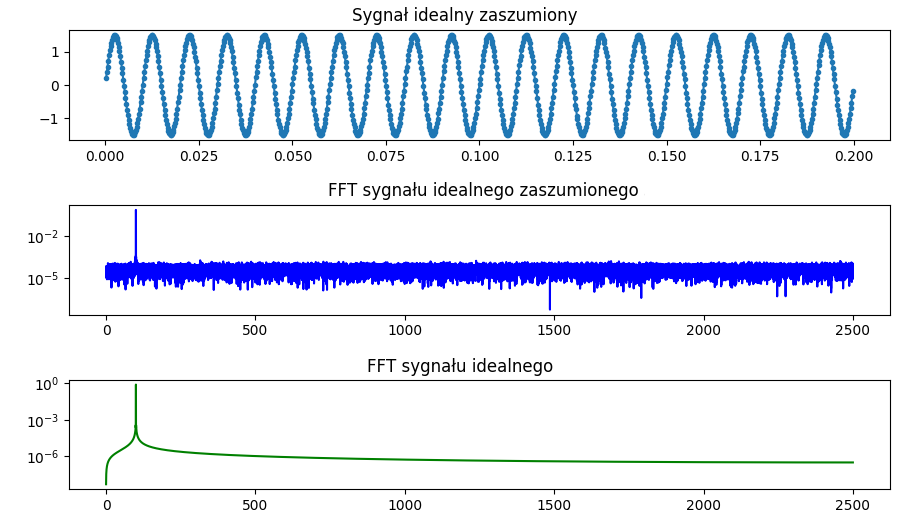
\includegraphics[width=14cm]{sin_fft_ideal}
	\caption{Analiza FFT dla sygnału sinus wygenerowanego numerycznie} 
	\label{fig:sin_fft_ideal}
\end{figure}

W celu zbadania stałości częstotliwości próbkowania przetwornika dokonano analizy FFT spróbkowanego sygnału. Rysunek \ref{fig:sin_fft_max1202} przedstawia przebieg czasowy otrzymany z 50000 próbek zebranych przetwornikiem ADC MAX1202, widmo sygnału spróbkowanego przemnożonego przez okno Hanning'a oraz charakterystyka częstotliwościowa sygnału sinusoidalnego wygenerowanego numerycznie.


\begin{figure}[H]
	%\centering
		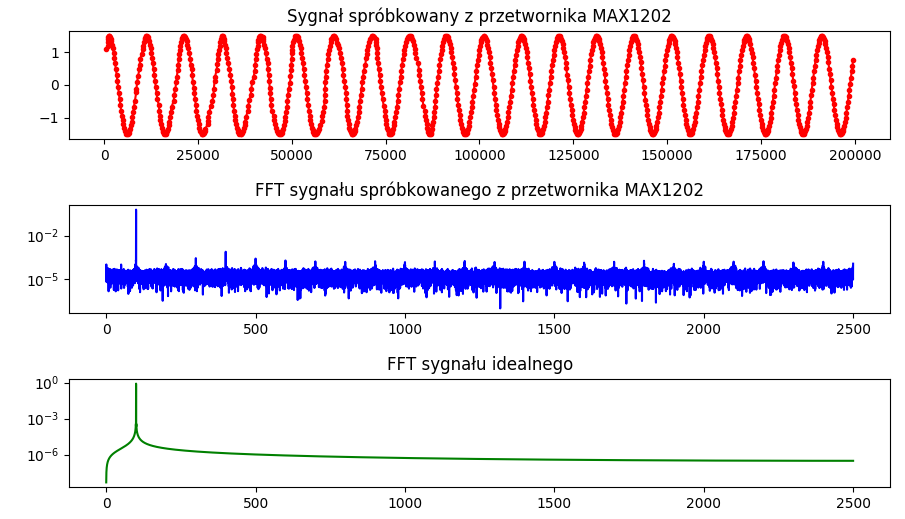
\includegraphics[width=14cm]{sin_fft_max1202}
	\caption{Analiza FFT dla sygnału spróbkowanego przetwornikiem ADC MAX1202} 
	\label{fig:sin_fft_max1202}
\end{figure}

\subsection{Pomiary ciśnienia czujnikiem LPS25H}

Zmierzono ciśnienie atmosferyczne w windzie gmachu Elektroniki i Technik Informacyjnych poruszającej się pomiędzy piętrami -2. i 4. zatrzymując się po drodze na 2. piętrze i na parterze. Na Rys. \ref{fig:winda} przedstawiono wyniki pomiarów. Jak widać na rysunku ciśnienie maleje zgodnie z wzorem barometrycznym wraz ze wzrostem wysokości. Po odpowiedniej kalibracji czujnik można wykorzystać do pomiaru wysokości.


\begin{figure}[H]
	\centering
		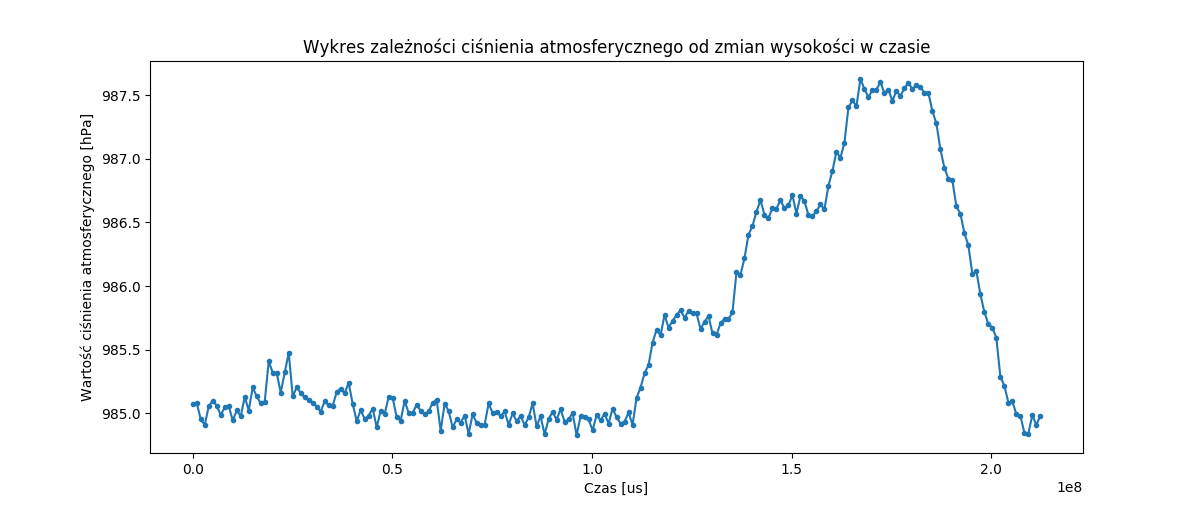
\includegraphics[width=14cm]{winda}
	\caption{Wykres zmian ciśnienia panującego w poruszającej się windzie} 
	\label{fig:winda}
\end{figure}


\section{Analiza wyników}
W celu dokonania porównania pomiaru maksymalnej częstotliwości próbkowania przeprowadzono analizę częstotliwościową spróbkowanego sygnału przy użyciu algorytmu FFT.
Zmienność częstotliwości próbkowania zobrazowano przy pomocy parametru odchylenia standardowego z poszczególnych odstępów czasowych pomiędzy momentami zebrania kolejnych próbek.

\begin{equation}
\sigma=\sqrt{\dfrac{1}{N}\sum_{0}^{N}{Var(x)}}
\end{equation}

x - odstępy pomiędzy momentami zebraniem próbki

N - ilość zebranych próbek


\subsection{Prezentacja i wizualizacja danych pomiarowych}
Optymalnym do tego zadania i znacznie ułatwiającym analizę wyników narzędziem był pakiet Pythona matplotlib. Są to pakiety zapewniające interfejs pozwalający na prezentację wyników w formie ułatwiającej analizę danych. Pliki z danymi ładowane były do aplikacji wyświetlającej wykresy w formacie pliku rozdzielanego przecinkami (csv).  



